\section{Introduction}

In this experiment we want to use the universal gas equation to determine the zero point of the so called thermodynamic Celsius temperature. 
In the process to find this coldest temperature possible in the absolute temperature, we use a glass bulb filled with helium,a pressure sensor and two well known temperatures to measure and calculate the zero point. 
Once the pressure and temperature of the helium in the glass bulb is know, all kinds of temperatures can be measured with the change of pressure in the sealed glass bulb.
To show this the temperature of liquid nitrogen is measured at the end of the experiment.
\begin{figure}[h]
	\centering
	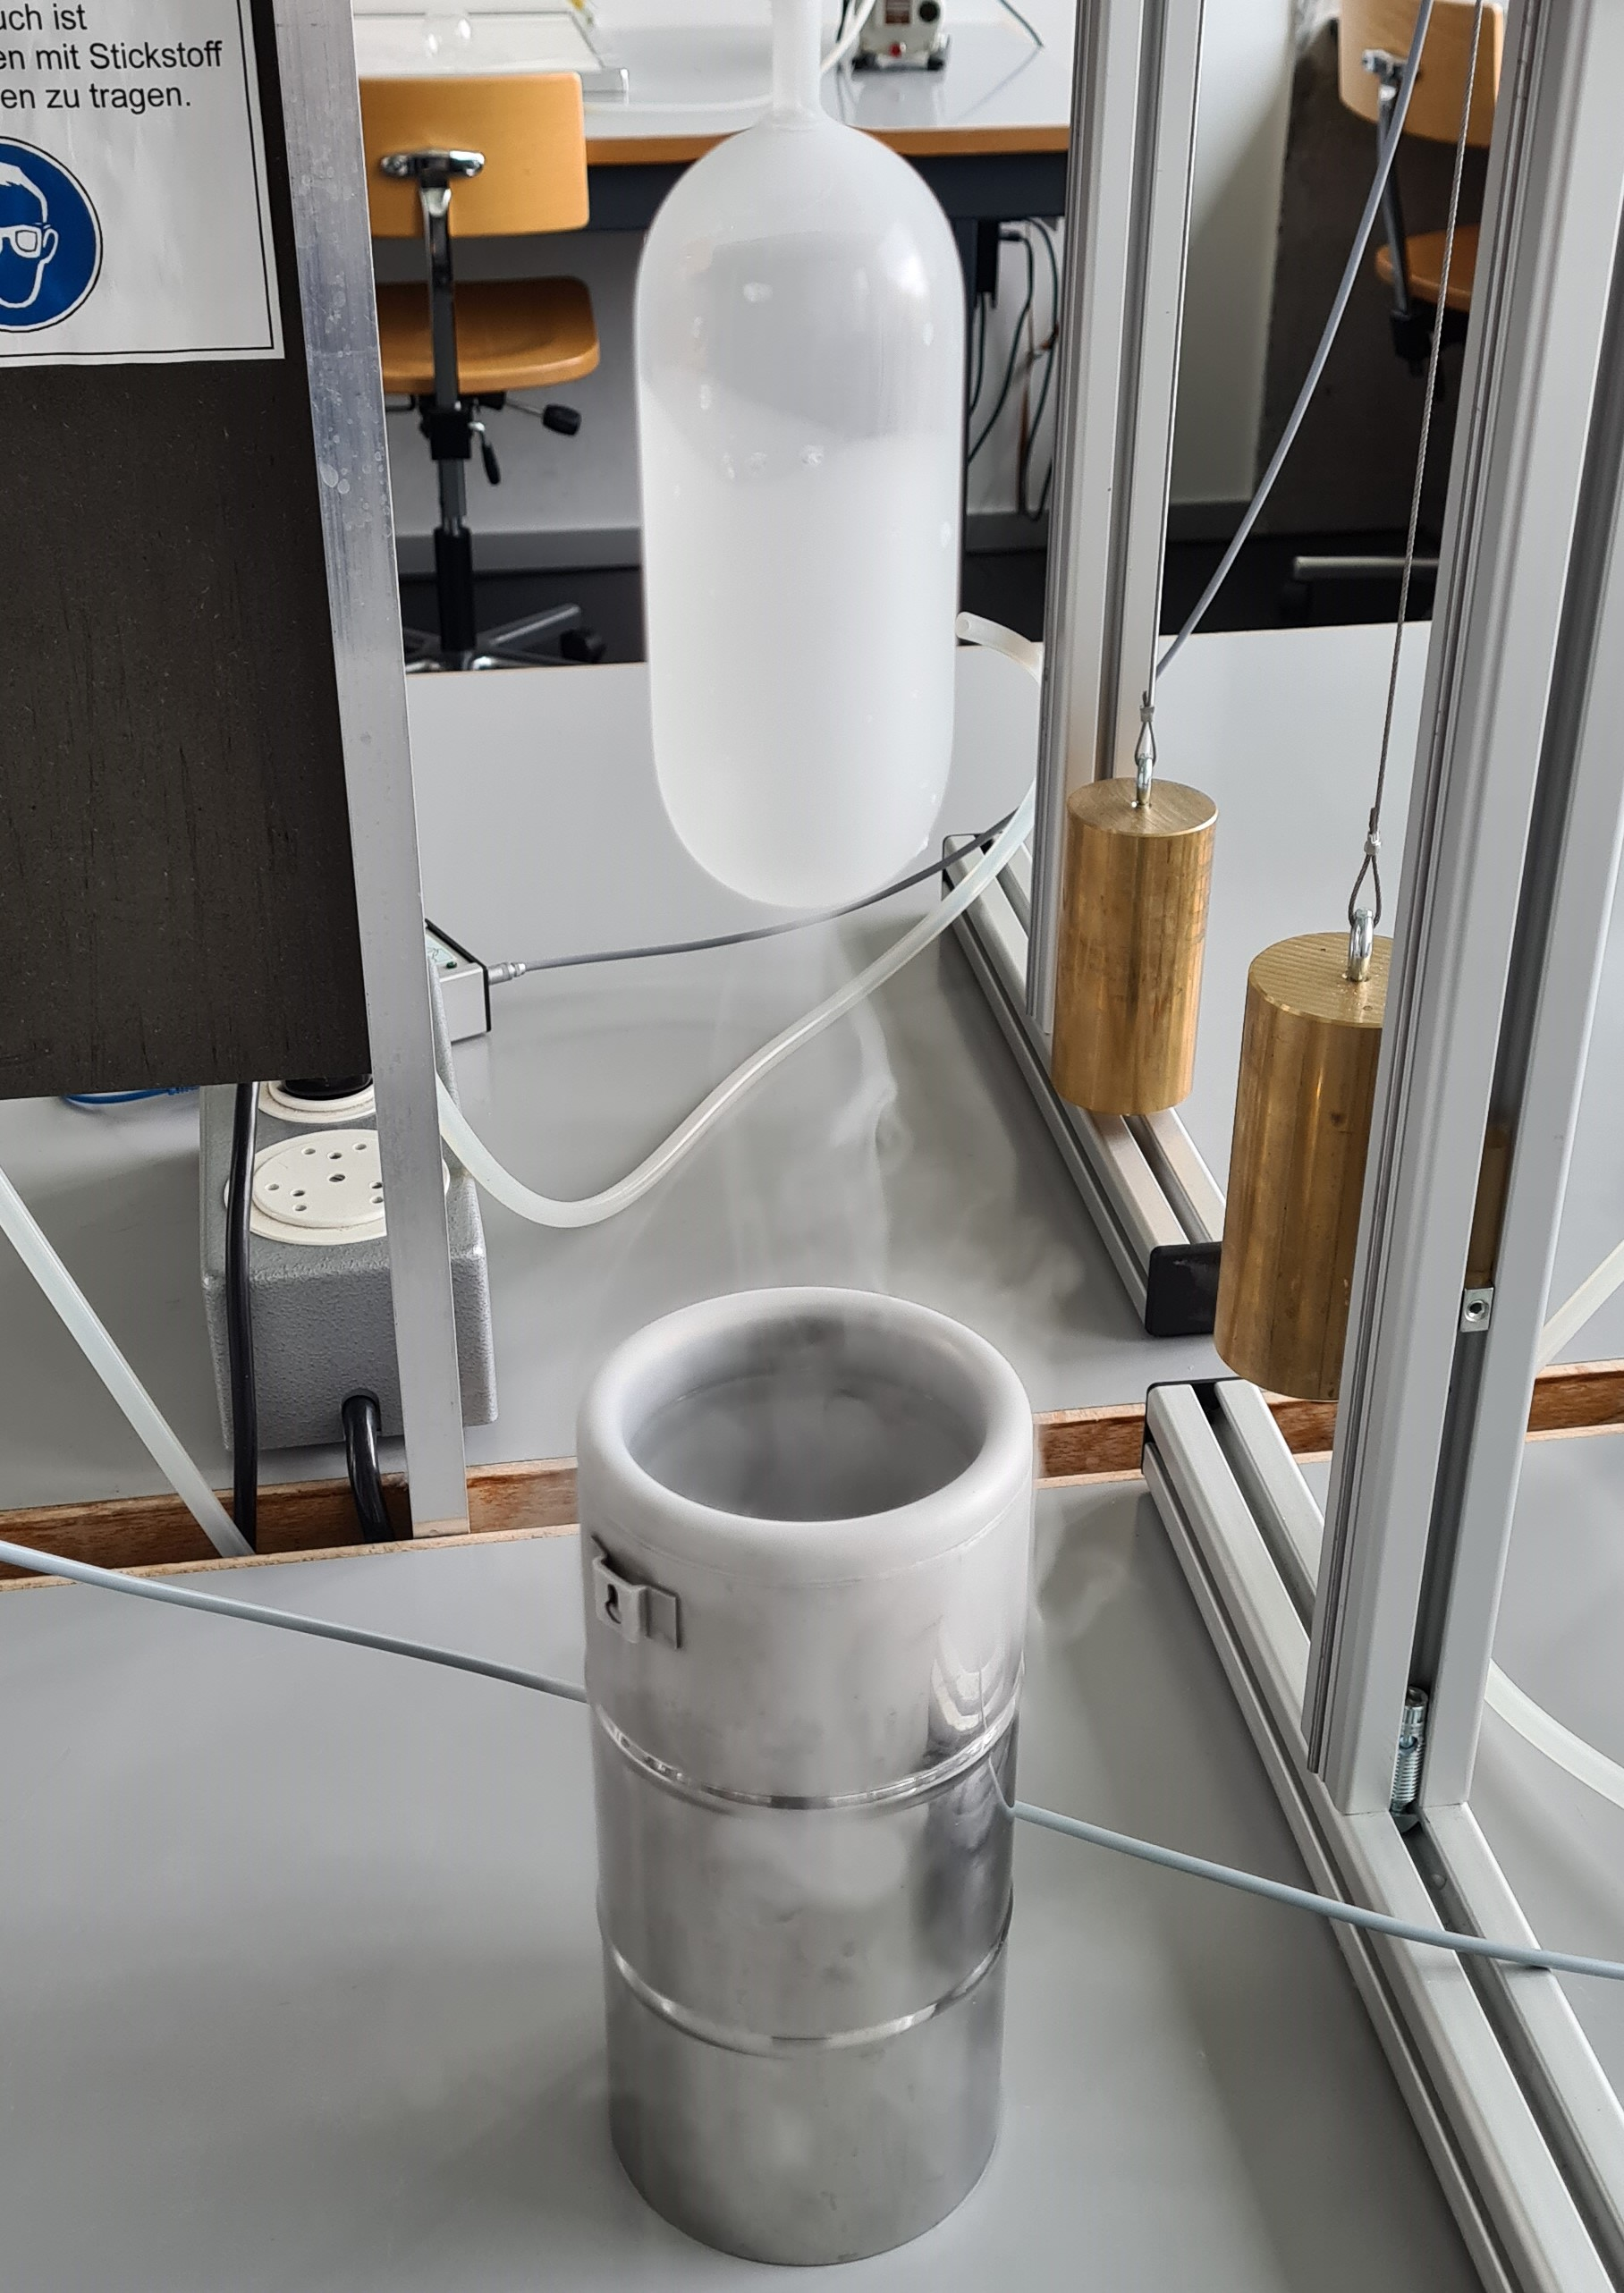
\includegraphics[width=0.5\textwidth]{sections/images/liquid.jpg}
	\caption{Sealed glass bulb filled with helium after being put in liquid nitrogen to measure the temperature of liquid nitrogen.}
\end{figure}
